\documentclass[journal]{IEEEtran}
\usepackage[a5paper, margin=10mm, onecolumn]{geometry}
\usepackage{tfrupee} % Include tfrupee package
\setlength{\headheight}{1cm} % Set the height of the header box
\setlength{\headsep}{0mm}     % Set the distance between the header box and the top of the text
\usepackage{xparse}
\usepackage{gvv-book}
\usepackage{gvv}
\usepackage{cite}
\usepackage{amsmath,amssymb,amsfonts,amsthm}
\usepackage{algorithmic}
\usepackage{graphicx}
\usepackage{textcomp}
\usepackage{xcolor}
\usepackage{txfonts}
\usepackage{listings}
\usepackage{enumitem}
\usepackage{mathtools}
\usepackage{gensymb}
\usepackage{comment}
\usepackage[breaklinks=true]{hyperref}
\usepackage{bookmark} % Add this line for better bookmarks management
\usepackage{caption} % Load the caption package with options
\usepackage{tkz-euclide}
\usepackage{color}
\usepackage{array}
\usepackage{longtable}
\usepackage{calc}
\usepackage{multirow}
\usepackage{hhline}
\usepackage{ifthen}
\usepackage{lscape}
\usepackage{float}
\renewcommand{\thefigure}{\theenumi}
\renewcommand{\thetable}{\theenumi}
\setlength{\intextsep}{10pt} % Space between text and floats
\numberwithin{equation}{enumi}
\numberwithin{figure}{enumi}
\renewcommand{\thetable}{\theenumi}

\begin{document}
\bibliographystyle{IEEEtran}
\title{9-9.3-13}
\author{EE24BTECH11030 - J.KEDARANANDA}
{\let\newpage\relax\maketitle}

\textbf{Question}:\\
Find the area bounded by the ellipse \(x^2 + 4y^2 = 16\) and the ordinates \(x = 0\) and \(x = 2\).

\solution

\begin{table}[h!]    
  \centering
  \begin{center}
    \begin{tabular}{|c|c|} 
        \hline
            \textbf{Variable} & \textbf{Value} \\ 
        \hline
            $\boldsymbol{BC}$ & 6 cm \\ 
        \hline
            $\boldsymbol{AB}$ & 5 cm \\ 
        \hline
            $\angle \vec{B}$  & $60^\circ$ \\
        \hline
    \end{tabular}
\end{center}  



  \caption{Variables Used}
  \label{tab1-1.9-6}
\end{table}

The equation of an ellipse in matrix form is
\begin{align}
\vec{x}^\top \vec{V} \vec{x} + 2 \vec{u}^\top \vec{x} + f = 0
\end{align}

The equation of a line in vector form is
\begin{align}
\vec{x} &= \vec{h} + \kappa \vec{m}
\end{align}

\begin{align}
\vec{V} &= \begin{pmatrix} \frac{1}{16} & 0 \\ 0 & \frac{1}{4} \end{pmatrix} \\
\vec{u} &= \begin{pmatrix} 0 \\ 0 \end{pmatrix} \\
f &= -1
\end{align}

For the given line \(x = 2\), the values of \(\vec{h}\) and \(\vec{m}\) are
\begin{align}
\vec{h} &= \begin{pmatrix} 0 \\ 0 \end{pmatrix} \\
\vec{m} &= \begin{pmatrix} 1 \\ 0 \end{pmatrix}
\end{align}

The intersection points are
\begin{align}
\vec{x_1} &= \begin{pmatrix} 2 \\ \sqrt{3} \end{pmatrix} \\
\vec{x_2} &= \begin{pmatrix} 2 \\ -\sqrt{3} \end{pmatrix} \\
\vec{x_3} &= \begin{pmatrix} 0 \\ 2 \end{pmatrix} \\
\vec{x_4} &= \begin{pmatrix} 0 \\ -2 \end{pmatrix}
\end{align}

The equation for \(y\) can be expressed as:
\begin{align}
y &= \pm \sqrt{4 - \frac{1}{4} x^2}
\end{align}

The area \(A\) between the curves from \(x = 0\) to \(x = 2\) is given by:
\begin{align}
A = 2 \int_0^2 \sqrt{4 - \frac{1}{4} x^2} \, dx
\end{align}

This simplifies to:
\begin{align}
A = 4 \int_0^2 \sqrt{1 - \frac{x^2}{16}} \, dx
\end{align}

Thus, the area becomes:
\begin{align}
A = 2\sqrt{3} + \frac{4\pi}{3}
\end{align}

\begin{figure}[!ht]
    \centering
    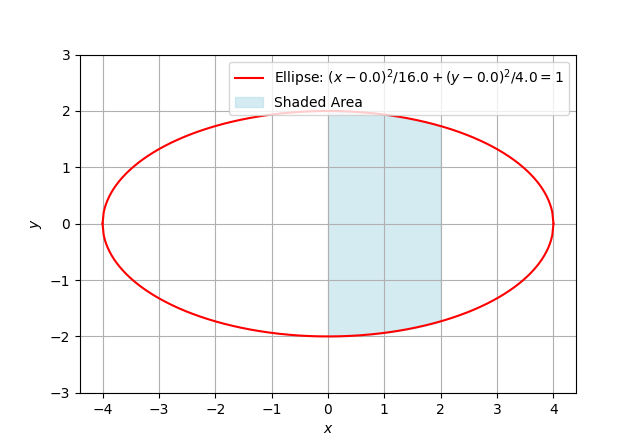
\includegraphics[width=\linewidth]{figs/fig1.png}
    \caption{Area Bounded by the Ellipse and the Ordinates}
\end{figure}

\end{document}

